\documentclass[a4paper,11pt]{article}
\usepackage[utf8]{inputenc}
\usepackage{eurosym}
\usepackage{graphicx}
\author{H.~Partl}
\title{Syntax of sec files}
\begin{document}
\maketitle
\tableofcontents
\begin{abstract}
Version 1.0

\end{abstract}
\section{Files}
A sec file is a plain text file.

\section{Format}
The format of the document is done with tabs, asterisks plus space and
white lines.

The indentation means importance. The more indentation the less 
important in the document structure.

The titles are formatted with one asterisks and one space.

\section{Structure}
\subsection{File}
A *.sec file is a Section.

\subsection{Section}
A section contains a title, zero or more paragraphs and zero or 
more subsections.

\subsection{Title}
A text string with no carriage return allowed.

\subsection{Paragraph}
The texts of the section.

The paragraphs can be:

\subsubsection{Normal paragraphs}
The first non-tab character can be any char except 
asterisk, slash or asterisk.

You can write a paragraph using many lines. 

To make a new paragraph, write a blank line.

The paragraphs are separated with blank lines.

\subsubsection{List elements}
The first non-tab character is a dash.

Example:

\begin{itemize}
\item  Europe
\item  America
\item  Asia
\end{itemize}
\subsubsection{Numeric list elements}
The first non-tab character is #

Example:

\begin{enumerate}
\item  Python
\item  C++
\item  Perl
\end{enumerate}
\subsubsection{Literal lines}
The first non-tab character is a greater-than sign.

Example:

\begin{verbatim}
class program:
  def run(self):
    print "Hello World"
    return 0
\end{verbatim}
\subsubsection{Definition lists}
You can do definition lists using List elements as term with the definition or definitions after two colons (::)

Example:

\begin{description}
\item[ title]
 Moby Dick
\item[ Author]
 Herman Melville
\item[ Year]
 1851
 1926, first movie
\end{description}
\subsection{Titles and Paragraphs }
Can contain:

\subsubsection{Plain text}
Plain text is..., well..., you know...

\subsubsection{Hyperlinks}
Hyperlinks are an URL and a title enclosed into double square
brackets, with an space between the URL and the title.

Example:

\begin{verbatim}
Search with [[http://www.google.es Google]].
\end{verbatim}
\subsubsection{Images}
You can include external and internal images with curly brackets.	

You can add optional elements as title and the URL for a bigger image.

Examples:

\begin{figure}[ht!]
		\centering
		\includegraphics[width=90mm]{http://sectxtweb.appspot.com/images/python_big.jpg}
		\caption{The python}
		\label{overflow}
		\end{figure}
		

\begin{figure}[ht!]
		\centering
		\includegraphics[width=90mm]{/images/python_big.jpg}
		\caption{The python with bigger image}
		\label{overflow}
		\end{figure}
		

\begin{figure}[ht!]
		\centering
		
\includegraphics[width=90mm]{/images/python.jpg}
		\caption{The python}
		\label{overflow}
		\end{figure}
		

\begin{figure}[ht!]
		\centering
		
\includegraphics[width=90mm]{/images/python.jpg}
		\label{overflow}
		\end{figure}
		

\subsection{Subsections}
The subsections are sections. Do you know what is recursion?

\end{document}
